\subsection{通信機,アンテナ概要}

本衛星に搭載する通信機としては,以下の3つがある.
\begin{itemize}
	\item {1} 地上局からのアップリンクを受信するVHF系
	\item {2} 地上局へCW信号,FM信号をダウンリンクするUHF系
	\item {3} 地上局へ大容量データをダウンリンクする5.8GHz系
\end{itemize}

衛星と地上局の通信の概略図を図\ref{fig4-2-1}に示す.
本衛星の回線設計は本衛星の軌道情報,東工大松永研究室地上局設備の性能を加味し,図\ref{fig4-2-2}のようになされた.
それぞれに要求される性能を記述する.
\begin{figure}[H]
	\centering
	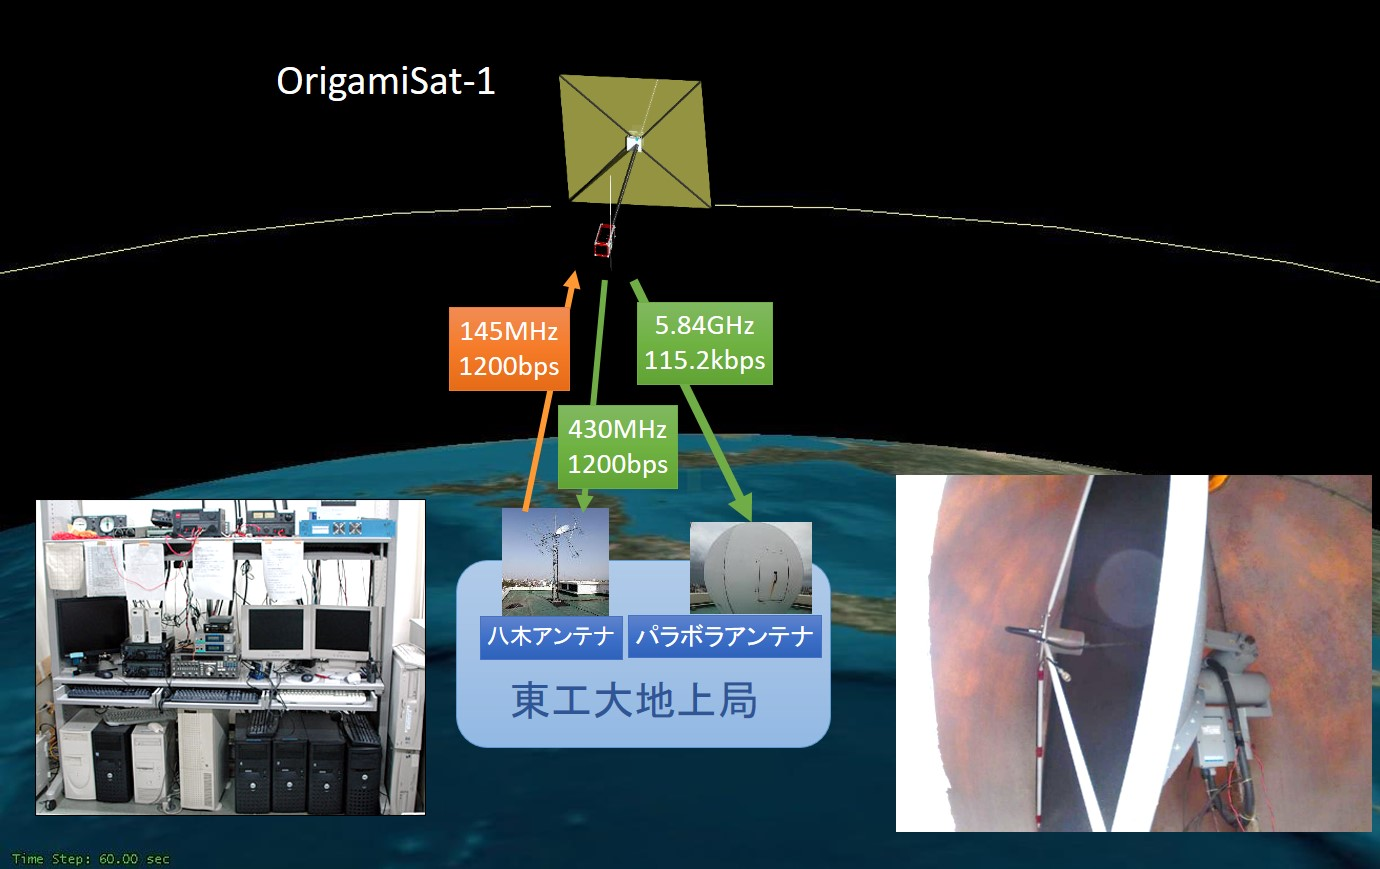
\includegraphics[scale=0.5]{03/fig/4-2-1.jpg}
	\caption{通信系概略図}
	\label{fig4-2-1}
\end{figure}
\begin{figure}[H]
	\centering
	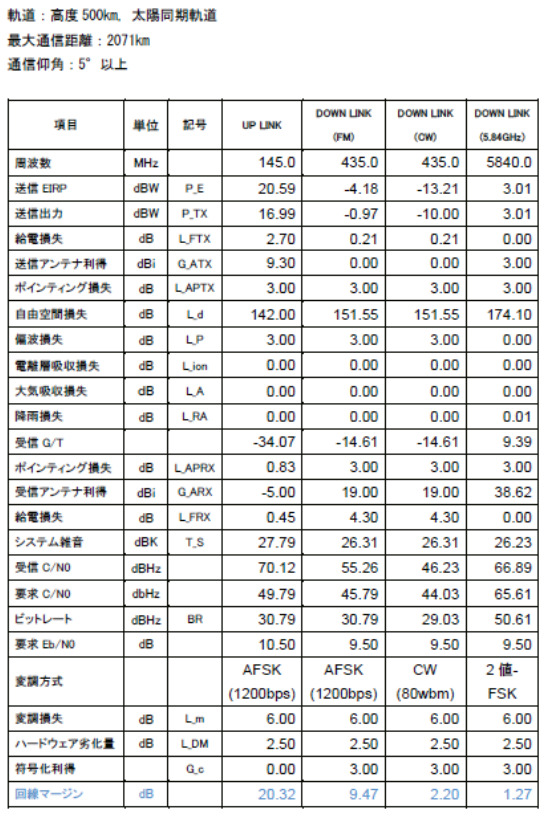
\includegraphics[scale=0.4]{03/fig/4-2-2.jpg}
	\caption{回線設計}
	\label{fig4-2-2}
\end{figure}

\subsection{VHF系}
VHF帯(Very High Frequency)の通信機では地上局からのアップリンクを受信するために用いる.通信機は西無線研究所の301A型(図\ref{fig4-2-ntrx})を用いた.
アンテナにはコンベックス加工を行ったリン青銅製のモノポールアンテナ(幅5mm, 厚さ0.1mm)のものを用い,長さはインピーダンスマッチング試験を通じて決定した.
以下に設計スペックおよび系統図(\ref{fig4-2-3})を示す.
\begin{itemize}
	\item 周波数:145.980MHz
	\item 送信出力:100mW(CW),800mW(CW)
	\item 寸法:60x50x10.5mm
	\item 重量:38g
	\item アンテナ利得:0dBi
	\item 周波数帯域幅:500Hz(CW),20kHz(FM)
\end{itemize}
\begin{figure}[htbp]
	\centering
	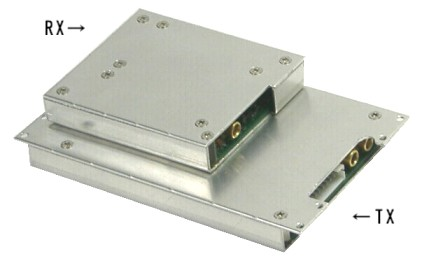
\includegraphics[width=0.5\linewidth]{03/fig/4-2-ntrx.jpg}
	\caption{TXE430MFMCW-301A, RXE145M-301A}
	\label{fig4-2-ntrx}
\end{figure}
\begin{figure}[H]
	\centering
	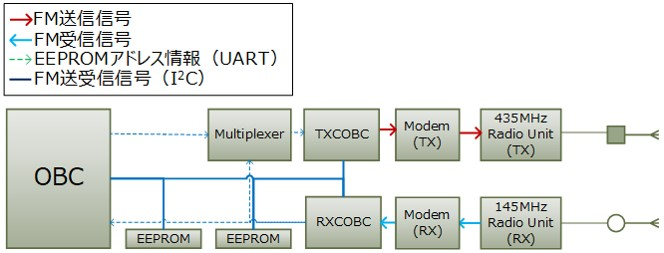
\includegraphics[scale=0.6]{03/fig/4-2-3.jpg}
	\caption{UHF/VHF系通信系統図}
	\label{fig4-2-3}
\end{figure}

購入した無線機内部にはモデム回路が組み込まれておらず,そのため本衛星ではCIB上にモデム回路が搭載された.
モデムICはCML Microcircuits社のFX614を購入した(購入先は誠大電機).初期はTexas Instruments社のTCM3105NLを用いて開発を行っていたが,調整必要なパラメータが大きくそれぞれの感度が高く送受信困難であったため,CubeSat仕様実績のあるFX614に変更した.モデム回路図を図\ref{fig4-4-2-rx_m}に示す.

\begin{figure}[htbp]
	\centering
	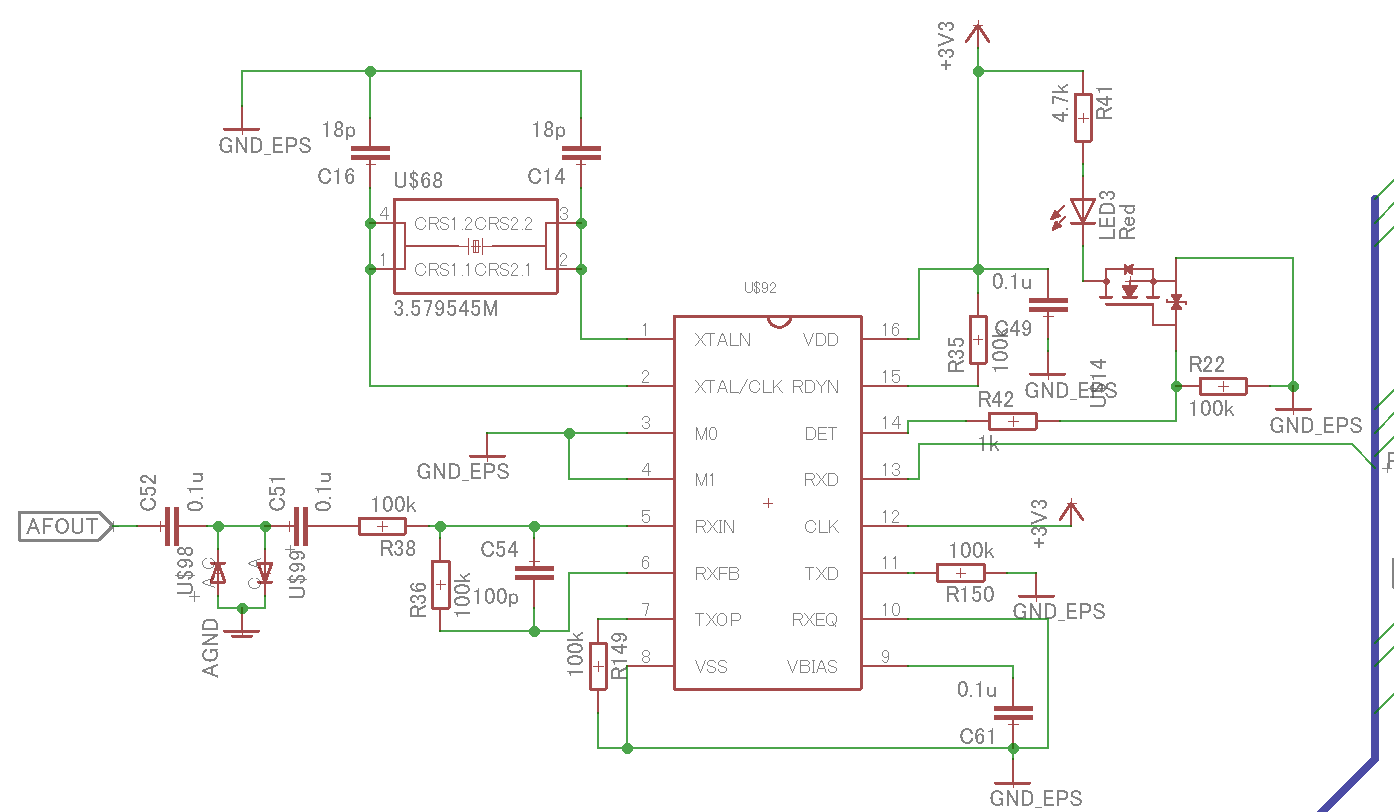
\includegraphics[width=0.7\linewidth]{03/fig/4-2-rx_modem.PNG}
	\caption{RX Modem Circuit Schematic}
	\label{fig4-4-2-rx_m}
\end{figure}



\subsection{UHF系}
UHF帯(Ultra High Frequency)の通信機では地上局へCW信号,FM信号をダウンリンクするために用いる.通信機は西無線研究所の301A型を用いた.
アンテナにはコンベックス加工を行ったリン青銅のモノポールアンテナ(幅5mm, 厚さ0.1mm)のものを用い,長さはインピーダンスマッチング試験を通じて決定した.
以下に設計スペックおよび系統図(\ref{fig4-2-3})を示す.
\begin{itemize}
	\item 周波数:437.505MHz
	\item 寸法:100x60x10.5mm
	\item 重量:60g
	\item アンテナ利得:0dBi
\end{itemize}




こちらもモデム回路はCIB上に新たに搭載された(図\ref{fig4-4-2-tx_m}).無線機のFMMOD端子には約0.5Vp-pのAFSK信号入力を推奨されていたため,この回路図のR155とR156の抵抗値は変更されるべきである.実験によってこの値でも問題なく通信できることは確認済であった.



\begin{figure}[htbp]
	\centering
	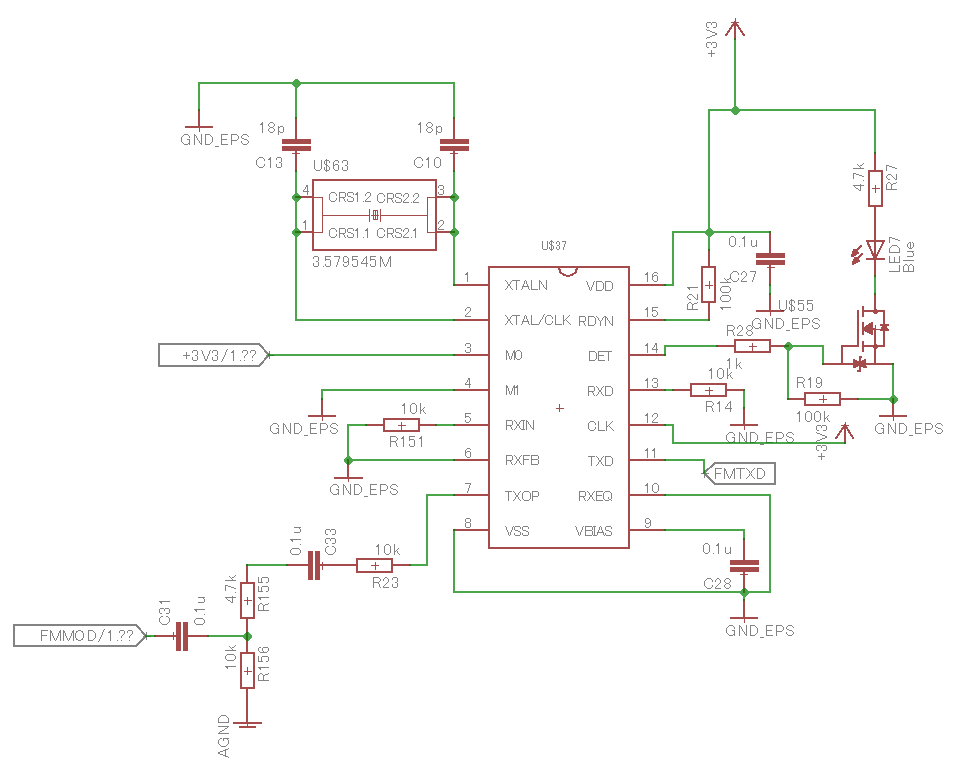
\includegraphics[width=0.7\linewidth]{03/fig/4-2-tx_modem.PNG}
	\caption{TX Modem Circuit Schematic}
	\label{fig4-4-2-tx_m}
\end{figure}




\subsection{5.8GHz系}
5.8GHz系の通信機では画像などの大容量データをダウンリンクするために用いる.通信機はロジカルプロダクト社製 LPTX5840-1を用いた.
アンテナには円偏波パッチアンテナ(30x30x1.6mm)を用いた.
以下に設計スペックおよび系統図(\ref{fig4-2-4})を示す.
\begin{itemize}
	\item 周波数:5840MHz
	\item 送信出力:2W
	\item 寸法:76x70x16mm
	\item 重量:220g
	\item アンテナ利得:3dBi
	\item 周波数帯域幅:210kHz
\end{itemize}
\begin{figure}[H]
	\centering
	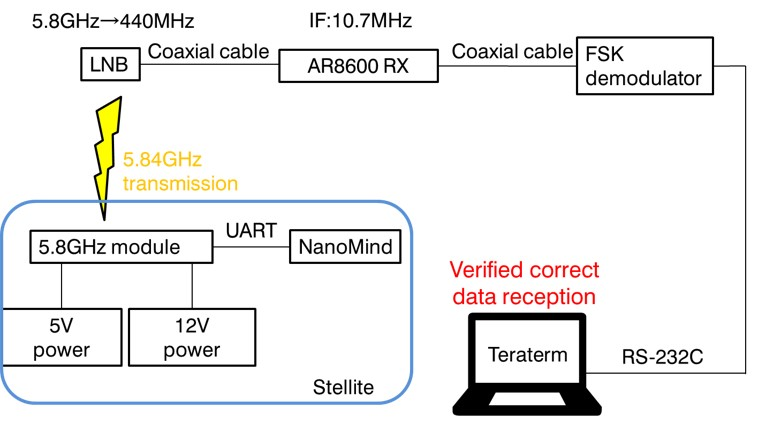
\includegraphics[scale=0.6]{03/fig/4-2-4.jpg}
	\caption{5.84GHz系通信系統図}
	\label{fig4-2-4}
\end{figure}

